\chapter{Reconstruction of Particle Properties using Machine Learning}\label{chp:reconstruction}

The final tasks of the event-wise analysis of \gls{iact} data is the estimation
of the physical properties of the measured events.
Three properties must be reconstructed to be able to perform physical analysis
of gamma-ray sources, e.\,g. measuring their spectral energy distribution:
\begin{description}
  \item[Particle type] As described in \autoref{sec:cosmic-rays}, \glspl{iact}
    measure thousands of air showers induced by charged cosmic rays for each
    measured gamma ray.
    To reduce this background as effectively as possible, events are classified
    as either gamma-ray or hadron induced.
    This is a classification task.
  \item[Primary energy] While techniques like unfolding could directly estimate
    a spectral distribution from several input features, condition of the inverse
    problem usually improves when using a direct estimator of the primary energy.
    This is a one-dimensional regression task.
  \item[Origin] The direction of origin also plays a crucial role in
    the background suppression, as the cosmic ray background is isotropic 
    compared to the compact or point-like gamma-ray sources.
    The two-dimensional regression to estimate the origin of a gamma ray
    is especially hard for monoscopic \glspl{iact}, as multiple telescopes
    allow simpler and more precise geometric reconstruction methods.
\end{description}

\noindent Historically, these tasks were performed by applying event selection criteria,
often called \emph{cuts}, for the particle classification and hand-crafted
regression formulas fitted to simulations for the energy estimation and reconstruction
of origin.
Modern methods of machine learning have improved performance and removed human biases
from these steps.

While there have been first successes \cite{hess_deep_learning,cta_index_dnn} in using convolutional neural networks
to directly reconstruct these properties from lower stages of the event 
processing\footnote{like the number of photons per pixel and their arrival time or 
even from the voltage time series in each pixel}, these analyses are all
in a prototype stage and seem much more dependent on mismatches between simulations
and observations than classical machine learning approaches using the image parameters
as input.
This is why the focus here will be laid to supervised, decision tree based ensemble methods.

For a long time, there has been no common file format or other representation of
reconstructed gamma-ray events, which could be used to enable analyses combining
multiple observatories. 
Each collaboration used their own file format and conventions.
An effort to standardize data formats for gamma-ray astronomy,
mainly in preparation for \gls{cta}—but also to enable joint analyses of the
currently operating telescopes—was started in 2015.
A first version of the specification based on the \gls{fits} standard has been published in 2016.~\cite{ogadf,ogadf-proceeding}.
This is an ongoing effort and part of this work was to enable the storage of \gls{fact}
reconstructed event lists in the new, open format.


\section{Supervised Machine Learning}
Machine learning is the process of finding an estimator $f$
for a quantity $Y$ given some inputs $X$ by using generic classes of estimators $f$
and fitting the parameters of these estimators by minimizing a loss-function.

In the following, I will use the notation which closely resembles the one used in
\cite{hasties}: The target property $Y$ of several observations will be represented
by the vector $\m{y}$.
The $p$ input quantities $X_j$ for these $N$ observations will be stored in the $N \times p$
Matrix $\m{X}$, where $\m{X}_{\bullet j}$ denotes the $j$-th column, all observations for
input quantity $X_j$ and $\m{X}_i$ denotes the $i$-th row, all input quantities for
observation $i$. 
For regression problems, where a continuous quantity is estimated, $Y$ is directly the target
variable.
For classification problems, where observations are to be sorted into different groups,
a target variable $\hat{Y}_g \in [0, 1]$ for each class $g$ is estimated and 
a sample is assigned class $\hat{G}_g$ if $\hat{Y}_g$ is greater than a prediction threshold $t_g$.
For binary classification, this simplifies to just predicting a single $\hat{Y}$ and using a single
\emph{prediction threshold} $t$ splitting the samples into two classes.

In supervised machine learning, the estimator's parameters are optimized on 
a dataset where the target variable $Y$ is known.
This is commonly called \emph{training}.
A trained estimator can then be used to predict $\hat{Y}$ for observations with unknown $Y$.

An important step is the validation of trained models on datasets that were not used
for the training but have known $Y$ to calculate quality metrics that compare the 
estimated quantity $\m{\hat{y}}$ with the true quantity $\m{y}$.
This is needed to prevent \emph{overfitting}, the effect that a model learns
the training dataset \enquote{by heart} instead of the underlying structure
and thus fails to generalize to data it has not been trained on.
Metrics and validation will be discussed in \autoref{sec:validation}.

Many different algorithms exist for both regression and classification tasks,
that differ greatly in their assumptions about the data, their generality, 
the loss-function they try to minimize.
Most algorithms are also tunable with so-called hyperparameters.
These are properties of the models that stay fixed for a single training
step but have to be optimized for the current application.
A simple example for a hyperparameter is the number of next neighbors $k$
considered in a $k$-Nearest-Neighbor classifier~\cite[chapter 9.1]{hasties}.
This all can greatly influence their quality metrics on a specific problem. 
In the following, I will introduce decision trees and random forests.
Random forests have proven to be a very general, robust, fast to train and fast to apply
model.
While boosting methods can often achieve slightly better performance, 
training time is usually much higher as their training cannot be parallelized.

\subsection{Decision Trees}

Decision trees locally optimize a loss function by recursively
splitting the feature space into subregions.
The most common case are binary trees, that in each step split each subregion
into two new regions.~\cite{cart}
Finding the optimal subdivision of a feature space using binary splits is
NP complete~\cite{trees_np}, so instead of finding \emph{the optimal} solution,
a greedy algorithm to find \emph{a good} solution is employed:
Starting from the full feature space $R$, the best split of all possible splits
in all $p$ features is done, splitting into two subspaces $R_1$ and $R_2$.
This procedure is repeated recursively in all resulting subspaces until a stopping criterion
is met, e.\,g.\ a maximum number of splits or a minimum number of samples in the
resulting subspaces. Each split is called a node, each final subspace is called a leaf.
For a regression tree, the output is the average of the training data in the leaf,
for classification, either the majority class or the partitions of the classes
in the leaf as continuous score ${} \in [0, 1]$ are returned.
The maximum number of splits is called the depth of the tree and can be used
to constrain the model complexity and thus overfitting.

For classification, there are two commonly used criteria to determine the best split, 
cross-entropy and the Gini-Index, which are pretty similar, for two classes
with $p$ being the proportion of one class, these are:
\begin{align}
  \text{Gini Index} &= 2p(1-p)\\
  \text{Cross-entropy} &= -p\log p - (1 - p) \log(1-p)
\end{align}
For regression, the mean squared error 
\begin{equation}
  \operatorname{mse} = \sum_{\mathclap{X_{ij} \, \in R_1}} (y_i - \hat{c}_1)^2
                     + \sum_{\mathclap{X_{ij} \, \in R_2}} (y_i - \hat{c}_2)^2
\end{equation}
is the most common loss function.
The criterion is evaluated for all possible splits in all features $X_j$ to find 
the best possible split for the current node. \cite[chapter 9.2]{hasties}

\subsection{Random Forests}

Because of the greedy algorithm, decision trees have intrinsically a high variance.
Small fluctuations in the training dataset can alter the very first splits and
thus alter the full tree.
To achieve a better and adjustable bias-variance-trade-off, Leo Breiman introduced
random forests~\cite{randomforest}.
A common approach to reduce variance is \emph{bagging}~\cite{bagging}. 
Multiple models are trained on slightly different datasets created by sampling with replacement from the original training dataset creating an ensemble.
For the final output, the outputs of the single models are averaged.
Random forests are a bagged ensemble of decision trees with an additional randomness
to further diversify the single decision trees: only a random subsample of the
features is considered for the best split in each node.

\subsection{Quality Metrics and Validation}\label{sec:validation}

\begin{figure}[tbp]
  \begin{captionbeside}{\label{fig:confusion}%
    Confusion for a binary classification problem.
    On the left are all samples belonging to the positive class, on
    the right the negative ones.
    The circle encompasses all samples classified as positive.
    This leaves us with four important areas, which are the entries in the
    confusion matrix. 
    Correctly classified positive samples are the true positives $\tp$,
    correctly classified negative samples are called true negative $\tn$.
    The falsely classified samples are called appropriately, short $\fn$ and $\fp$.
    The confusion matrix is then
    \begin{equation}
      \begin{pmatrix}\tp & \fp \\ \fn & \tn \end{pmatrix}.
    \end{equation}
    Adapted from \cite{confusion-matrix}.
  }%
    \raisebox{\dimexpr\baselineskip-\totalheight\relax}{%
      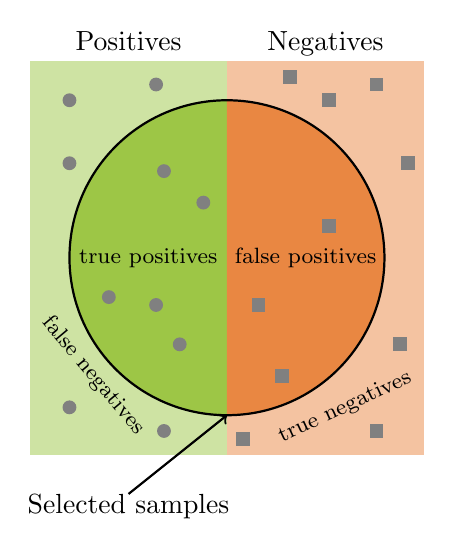
\begin{tikzpicture}
  \tikzset{every node/.style={inner sep=0,outer sep=0}}

  \definecolor{positive}{RGB}{132, 184, 24}
  \definecolor{negative}{RGB}{227, 105, 19}

  \node[above] at (1.25, 5) {\strut Positives};
  \begin{scope}
    \clip (0, 0) rectangle (2.5, 5);
    \fill[positive!40] (0, 0) rectangle (2.5, 5);
    \fill[positive!80] (2.5, 2.5) circle [radius=2];
  \end{scope}


  \node[above] at (3.75, 5) {\strut Negatives};
  \begin{scope}
    \clip (5, 0) rectangle (2.5, 5);
    \fill[negative!40] (5, 0) rectangle (2.5, 5);
    \fill[negative!80] (2.5, 2.5) circle [radius=2];
  \end{scope}

  \draw[thick] (2.5, 2.5) circle [radius=2];

  \foreach \xy in {
    (0.5, 0.6), (0.5, 4.5), (1.7, 3.6), (1., 2.0), (0.5, 3.7),
    (1.6, 4.7), (1.9, 1.4), (2.2, 3.2), (1.6, 1.9), (1.7, 0.3)
  } {
    \node[fill=gray, circle, minimum size=5pt] at \xy {};
  }
  \foreach \xy in {
    (3.8, 2.9), (4.4, 0.3), (3.8, 4.5), (4.4, 4.7), (4.7, 1.4),
    (2.9, 1.9), (3.3, 4.8), (3.2, 1.0), (4.8, 3.7), (2.7, 0.2)
  } {
    \node[fill=gray, rectangle, minimum size=5pt] at \xy {};
  }
  \draw[thick, <-] (2.5, 0.5) -- (1.25, -0.5) node[below]{Selected samples};
  \node[] at (1.5, 2.5) {\footnotesize true positives};
  \node[] at (3.5, 2.5) {\footnotesize false positives};
  \node[rotate=25] at (4, 0.6) {\footnotesize true negatives};
  \node[rotate=-50] at (0.8, 1.0) {\footnotesize false negatives};
\end{tikzpicture}
%
    }% 
  \end{captionbeside}
\end{figure}

There are two different quality metrics relevant for the evaluation of
the models trained to perform \gls{iact} event reconstruction.
In this section, I will focus on quality metrics commonly used in statistics
and machine learning for the evaluation of classifiers and regressors.
The quality metrics commonly used in gamma-ray astronomy to describe
the performance of the full analysis chain of an \gls{iact} will be discussed
in \autoref{chp:performance}.
All quality metrics for binary classification build upon the confusion matrix,
a visual explanation of which is shown in \autoref{fig:confusion}.
The most common quality metrics for binary classification are:
\begin{description}
  \item[Precision] also referred to as purity or positive predictive value,
    is the percentage of positive samples in the selected samples:
    \begin{equation}
      \precision = \frac{\tp}{\tp + \fp}.
    \end{equation}
  \item[Recall] also known as true positive rate, efficiency or sensitivity, is the fraction 
    of selected positive samples to all positive samples:
    \begin{equation}
      \recall = \frac{\tp}{\tp + \fn}.
    \end{equation}
  \item[Accuracy] is the fraction of correctly classified samples
    \begin{equation}
      \operatorname{accuracy} = \frac{\tp + \tn}{\tp + \tn + \fp + \fn}
    \end{equation}
  \item[F-Score] is the harmonic mean of $\precision$ and $\recall$,
    where the weight $β$ can be used to put more emphasize on recall ($β < 1$)
    or precision ($β > 1$):
    \begin{equation}
      f_β = (1 + β²) \frac{\precision \cdot \recall}{β² \precision + \recall}
    \end{equation}
\end{description}

\begin{figure}
  \begin{captionbeside}{%
      \gls{roc} curves for three different classifiers for a simple toy example.
      The perfect classifier creates a square, as $\tpr = 1, \fpr = 0 \, \forall t_p > 0$
      and has $\AROC = 1$.
      Randomly guessing yields the diagonal and thus $\AROC = \num{0.5}$.
      Any classifier performing better than guessing $\hat{Y}$ uniformly will
      have $\num{0.5} < \AROC < \num{1}$.
    }
    \raisebox{\dimexpr\baselineskip-\totalheight\relax}{%
      \includegraphics{build/plots/roc_example.pdf}%
    }%
  \end{captionbeside}\label{fig:roc-example}
\end{figure}


All theses metrics require the classification into the classes $\hat{G}$.
As most models provide a score $\hat{Y}$, it is often useful to optimize
model hyperparameters on a metric that uses $\hat{Y}$, so that 
the optimization of model hyperparameters is independent of the optimization
of the prediction threshold $t_p$.
In the \gls{roc} curve~\cite{roc}, the true positive rate ($\operatorname{tpr}$) is
plotted against the false positive rate ($\operatorname{fpr}$) for all possible thresholds $t_p$.
The area under this \gls{roc} curve \AROC{} is a metric that describes
classifier performance independent of $t_p$ with a single number and
is thus a common metric for the optimization of hyperparameters.
Three prototypical cases for \gls{roc} curves are shown in \autoref{fig:roc-example}.
The \gls{roc} curve is also independent of the class balance.

For regression problems, the mean squared error is a commonly used metric,
but it is a highly problem specific one.
A generalization is the \emph{coefficient of determination} or $r²$-score,
which is defined as
\begin{equation}
  r² = 1 - \frac{\sum_{i=0}^N ({y_i - \hat{y}_i})^2}{\sum_{i=0}^N (y_i - \bar{y})^2},
\end{equation}
where $\bar{y}$ is the arithmetic mean of all $y_i$.
This metric is $1$ for the perfect regressor, $0$ for a regressor always
predicting $\bar{y}$ and $< 0$ for any regressor doing worse than simply predicting
the mean.

All metrics have limited informative value without considering how they depend
on the statistical fluctuations of training and application dataset.
A common method to not jeopardize the available data for training too much by splitting
into independent training and test sets, is cross validation.
Here, a dataset is split into $N$ parts but training happens $N$ times
on $N - 1$ parts and testing and metric evaluation is done on the remaining part.
Thus all test parts are independent, but the training data is overlapping and
each sample in the training data is used for evaluation exactly once.


\subsection{The \texttt{aict-tools}}

To be able to train, validate and apply models using supervised machine learning
to \gls{iact} data, the \texttt{aict-tools}~\cite{aict-tools} have been developed.
This python package provides command line utilities to train and apply models from
the \texttt{scikit-learn}~\cite{scikit-learn} library to image parameters of
\gls{iact} events stored in columnar oriented \texttt{hdf5}~\cite{hdf5} files.

Models provided by \texttt{scikit-learn} include linear regression, 
naive Bayes, support vector machines, tree based algorithms and ensemble 
learners, for example random forests and several versions of boosted decision trees.

The models are configured using \texttt{yaml}-Files~\cite{yaml}, a human and 
machine readable, plain-text data format. 
An example configuration for an energy estimation using a linear regression
of five features is shown in \autoref{lst:energy-example}.

\begin{lstlisting}[
  caption={%
    Example \texttt{aict-tools} configuration for an energy estimation using
    \texttt{scikit-learn}'s linear regression.
  },
  label={lst:energy-example},
  float
]
seed: 0 # seed for the random number generators

energy:
  regressor : linear_model.LinearRegression()

  n_signal: 50000
  n_cross_validations: 10

  target_column: corsika_event_header_total_energy
  output_name: gamma_energy
  log_target: True

  features:
    - size
    - length
    - width
    - leakage1
    - leakage2
\end{lstlisting}

Models are serialized for later application using either \texttt{joblib}~\cite{joblib},
which is an efficient storage format for Python classes containing large arrays, or
one of two language independent, standardized formats for machine learning models:
\gls{pmml}~\cite{pmml} or the ML extension for classical machine learning models of the \gls{onnx}~\cite{onnx}.
This can be used to apply models trained using \texttt{aict-tools} using 
other programming languages and tools, for example in \texttt{FACT-Tools}~\cite{streaming_adass}.

Three pairs of \texttt{aict\_train\_} and \texttt{aict\_test\_} programs are 
provided for the particle classification, the energy estimation and the
reconstruction of origin using the disp method, respectively.

The project was started by Kai Brügge in 2016 and I joined in early 2017, 
when only energy estimation and particle classification were implemented.
The main focus at the time was to replace the RapidMiner~\cite{rapidminer} based
analysis developed in \cite{phd-temme}, with some key points in mind:
\begin{itemize}[nosep]
  \item Better reproducibility through simple configuration files in text format
    compared to the GUI based RapidMiner approach.
  \item Better performance for application to larger datasets.
    Training and application times of the Weka random forest in RapidMiner
    were much larger than for the \texttt{scikit-learn} random forest.
  \item No dependencies on closed source, proprietary software\footnote{While RapidMiner is
    open core, the free version has a limitation of only \num{10000} rows for datasets
    and can also only utilize one CPU core.}.
\end{itemize}
Later, as one major part of the work done for this thesis, I developed and
implemented the origin reconstruction into the \texttt{aict-tools} based on
the disp method~\cite{disp} which is explained in detail in \autoref{sec:origin}.

In addition to the tools for model training and application, the \texttt{aict-tools} also
provide  utilities to
\begin{itemize}[nosep]
  \item apply event selection cuts, also configured via a \texttt{yaml} file,
  \item split datasets into multiple subsets, \eg for training and testing,
  \item create plots of quality metrics to evaluate model performance.
\end{itemize}

\section{Particle Classification}\label{sec:classification}

Particle classification is done using a random forest classifier trained
to distinguish gamma-ray induced showers (signal) from proton induced
showers (background). 

The output is called \param{gamma\_prediction}, with values close to \num{1} indicating
a shower likely induced by a gamma ray.
Compared to the previous, RapidMiner based analysis in \cite{phd-temme}, all
features depending on the known position of a point source were excluded from 
the training because of three reasons:
\begin{itemize}
  \item It greatly simplifies application of the models as they only have to be evaluated
    once and not for each of the on and off positions using the feature set for the 
    corresponding position.
  \item It enables predicting a single reconstructed position for each event on the sky
    completely independent of any assumptions about any source.
  \item It separates the two tasks of estimation of origin and particle classification.
    In \cite{phd-temme}, because the distance to the assumed source position was used
    for the classification, these steps were intertwined.
\end{itemize}

The second reason is important for the creation of skymaps or in cases where
no source position is known precisely or at all, e.\,g.\ when \gls{fact} performs
follow-up observations of alerts by the IceCube experiment, where the neutrino 
direction typically has uncertainties in the order of \SI{1}{\degree} \cite{icecube-hese}.
This is also the reason, why training is now done using diffuse gamma rays instead
of gamma rays observed in wobble mode.
Using diffuse gamma rays, the model should be able to better generalize in 
separating gammas from protons, and not just selecting events close to the wobble radius.

\section{Energy Estimation}

Energy estimation is done using a random forest regressor trained
to predict the natural logarithm of the energy with the \gls{mse} as loss function.
The choice of using the logarithm as opposed to the value itself is motivated in
the large domain of the primary energies.
The loss function would be completely dominated by few very high energy events
if evaluated on the values themselves.
Using the logarithm of the energy, the lower energy particles also contribute to
the loss and overall performance over the whole energy range is improved.

\section{Origin Estimation}\label{sec:origin}

In general, the estimation of the gamma ray origin is a two dimensional regression
task, as either two coordinates in the detector plane or on the sky
have to be estimated. 
To simplify the task, the assumption is made, that the source position lies
on the reconstructed shower axis. 
While this introduces a source of error if the shower axis is not properly reconstructed,
this simplifies the task from a two dimensional regression to a one dimensional regression
and a classification task.
The objective of the regression task is to find the absolute distance from the
center of gravity of the shower image to the origin of the shower called \param{disp} and the
classification task is to find the direction on the shower axis, which can be
interpreted as the sign of \param{disp}. 
This is also referred to as \enquote{head-tail-disambiguation} and is shown in \autoref{fig:head-tail}.

\begin{figure}
  \centering
  \includegraphics{build/plots/hillas_disp.pdf}
  \caption{%
    The two possible reconstructed source positions for a given $\abs{\param{disp}}$,
    the selection of the correct one is the target of the head-tail disambiguation.
  }\label{fig:head-tail}
\end{figure}

This method was developed for the Whipple telescope~\cite{disp}, greatly improving
the sensitivity for point sources over the methods used before, that did not predict
a source position at all but only used the orientation of the Hillas ellipse.
Disp was parameterized using
\begin{equation}
  \param{disp} = \xi \left(1 - \frac{\param{width}}{\param{length}}\right), \quad \text{\cite[(7)]{disp}}\label{eq:disp}
\end{equation}
which is also the parameterization used by the \facttools{} analysis.
The parameter $\xi$ was found either by optimizing it on observed data of a known, 
strong source as in \cite{disp} or on simulations as for the \facttools{}.
As this parameter $\xi$ is just a fixed number, \eqref{eq:disp} is not able
to predict $\abs{\param{disp}}$ well over a large energy range.
The value used in the \facttools{}, $\xi = \SI{1.38}{\degree}$, performed best
around an energy of \SI{3}{\TeV}, see \autoref{fig:ang-comp}, but much worse at higher energies.
The \facttools{} head-tail-disambiguation used features dependent on the known position
of a point-source. 
While this greatly increased the efficiency of the prediction—especially for low energy
gamma rays—it also increased the false positive rate as all showers including
the diffuse hadronic background were more often predicted towards the suspected gamma source.
The other drawbacks of using source-dependent image features discussed in \autoref{sec:classification} also apply here.
As the prediction is not independent of the source position, it has to be repeated for
the off positions, increasing the computational costs with each off position.
It also prevents the creation of skymaps, as there is no single prediction 
for an event.

\begin{figure}
  \centering
  \includegraphics{build/plots/hillas_true_disp.pdf}
  \caption{%
    The two possibilities for choosing the label for training the disp regression.
    The gray line shows the distance from the cog to the source position, the
    blue line shows the projection onto the reconstructed shower axis.
  }\label{fig:true-disp}
\end{figure}

The \gls{magic} experiment improved upon the simple parameterization in \eqref{eq:disp} using parameters
  depending on image parameters, e.\,g.\ \param{size},
to model energy dependencies and \param{leakage} to better handle showers
not fully contained in the camera~\cite{magic-disp}.
Finally in 2009, before \gls{magic}-II was built and \gls{magic} thus moved
to stereo reconstruction techniques, using a random forest regressor to estimate 
$\abs{\param{disp}}$ was evaluated and found to perform better than the previous parameterization~\cite{magic-disp-rf}.
In that case, the prediction for $\sgn{\param{disp}}$ was done using the difference between the image center
of gravity and its brightest pixel, which is related to the skewness of the light distribution.
To adapt these methods for the \facttools{} analysis chain, the \param{disp} estimation
was built into the \texttt{aict-tools}.
To further improve over previous works, a random forest classifier is employed
for the head-tail-disambiguation.
This results in a single prediction of origin for each event in the
detector coordinates frame, which can be transformed
to a position in the \gls{icrs} as described in \autoref{sec:coordinate-transforms}.
The predicted source position can be used to create skymaps and is also mandatory 
in the \gls{oga} fits format~\cite{ogadf} for \gls{iact} event lists.

As the determination of the shower axis is not always perfect,
there are two possibilities for the training of the disp regression.
The first is to assume \param{delta} is correct and just use the distance of the 
source position to the center of gravity.
The second is to transform the source position into the shower coordinate system 
and taking the coordinate along the main axis as disp.
Both versions are the same if \param{delta} has no error.
This is visualized in \autoref{fig:true-disp}.
It was found that the two differences do not differ in their results significantly
and the first version was chosen.
